% Slides for coauthors: the model after the fresh look ("Matsuyama in space").
% Compile with XeLaTeX (Fira fonts) from docs/slides/:
%   latexmk -xelatex matsuyama_in_space.tex
% Figure: python docs/slides/make_figures.py (from the repository root).
\documentclass[10pt,aspectratio=169]{beamer}

\usetheme[progressbar=frametitle,block=fill,numbering=fraction]{metropolis}
\usepackage{appendixnumberbeamer}
\usepackage{booktabs}
\usepackage{array}
\newcolumntype{L}[1]{>{\raggedright\arraybackslash}p{#1}}
\usepackage{amsmath,amssymb,mathtools}
\usepackage{bm}
\usepackage{tikz}
\usetikzlibrary{arrows.meta,positioning,shapes.misc,fit,backgrounds,calc}
\usepackage{pgfplots}
\pgfplotsset{compat=1.18}
\usepackage{xcolor}

\definecolor{mDarkTeal}{HTML}{23373B}
\definecolor{mOrange}{HTML}{EB811B}
\definecolor{mGreen}{HTML}{14B03D}
\definecolor{mLight}{HTML}{EEEEEE}
\newcommand{\hl}[1]{\textcolor{mOrange}{#1}}
\newcommand{\mute}[1]{\textcolor{gray}{#1}}
\newcommand{\unv}{$^{\dagger}$}
\setbeamerfont{footnote}{size=\tiny}

\tikzset{
  box/.style={draw=mDarkTeal, rounded corners=2pt, fill=mLight, align=center,
              font=\scriptsize, inner sep=4pt, text width=#1},
  box/.default=3cm,
  hot/.style={draw=mOrange, fill=mOrange!12, line width=0.8pt},
  arr/.style={-{Stealth[length=5pt]}, mDarkTeal, line width=0.7pt},
}

\title{Matsuyama in Space}
\subtitle{Agriculture, connectivity and Korea's escape from poverty, 1965--85\\
\small Where the model stands after the fresh look}
\author{Korea growth project --- working slides for coauthors}
\date{4 October 2026}

\begin{document}

\maketitle

\begin{frame}{Roadmap}
  \setbeamertemplate{section in toc}[sections numbered]
  \tableofcontents[hideallsubsections]
  \vfill
  \begin{block}{One-line summary}
    We re-centred the project on the \emph{macro} story. The baseline is now Korea's
    1965--85 history, and the core mechanism is a spatial version of Matsuyama (1992):
    whether farm productivity growth \hl{retains} or \hl{releases} labour depends on each
    township's access to crop markets and to non-farm jobs.
  \end{block}
\end{frame}

% =====================================================================
\section{Narrative}
% =====================================================================

\begin{frame}{The question}
  \textbf{How did Korea escape poverty between 1960 and 1990, and through which mechanisms?}
  Candidates: industrial parks, roads, rural transformation, world demand, capital, schooling.
  \vspace{0.6em}

  \begin{columns}[T]
    \begin{column}{0.6\textwidth}
      \scriptsize
      \begin{tabular}{@{}lll@{}}
        \toprule
        Margin & $\sim$1960/65 & $\sim$1980/90 \\
        \midrule
        Real GDP per capita & 1 & $\times$4 (1985)\unv \\
        Agriculture, employment share & 59\% (1965)\unv & 25\% (1985)\unv \\
        Manufacturing, VA share & 15\% (1965) & 30\% (1985) \\
        Urban population share & 28\% (1960) & 57\% (1980), 74\% (1990) \\
        Farm household population & $\sim$14m & $<$6m (1990) \\
        Exports / GDP & $\sim$9\% (1965)\unv & $\sim$33\% (1985)\unv \\
        Absolute poverty & $\sim$2/5 (mid-60s)\unv & $\sim$1/10 (1980)\unv \\
        \bottomrule
      \end{tabular}\\[0.3em]
      \tiny Unmarked: paper draft / WDI. \unv{} order-of-magnitude values, not yet checked
      against source (\texttt{scripts/data\_targets.py}).
    \end{column}
    \begin{column}{0.36\textwidth}
      \small
      \begin{itemize}
        \item One of the fastest structural transformations on record.
        \item Poverty was overwhelmingly \hl{rural}: the countryside is where parks, roads
              and rural programmes should matter most.
        \item The township panel being digitised (1960--90, annual) lets us see the
              transformation \emph{where it happened}.
      \end{itemize}
    \end{column}
  \end{columns}
\end{frame}

\begin{frame}{From ``perturb a stationary economy'' to ``subtract from history''}
  \begin{columns}[T]
    \begin{column}{0.48\textwidth}
      \textbf{Old design}\\[0.2em]
      \footnotesize
      Calibrate a 1965 economy, switch on HCI, report policy $-$ baseline.\\[0.4em]
      What the fresh look found when the code was run against the macro story:
      \begin{itemize}\footnotesize
        \item Trade closure was \hl{indeterminate}: wages differing by 65\% all solved to
              $10^{-12}$.
        \item 1965 economy not Korea: exports 73\% of GDP, farm employment 11\%.
        \item \hl{No growth engine}: baseline GDP $\times$1.12 over 1965--85 (data $\times$4);
              HCI supplied $\sim$2/3 of all model growth.
        \item Mechanisation and export margins un-nested; agriculture at a corner.
      \end{itemize}
    \end{column}
    \begin{column}{0.48\textwidth}
      \textbf{New design: baseline = history}\\[0.2em]
      \footnotesize
      \begin{itemize}
        \item The baseline reproduces the observed transformation.
        \item Programmes enter as \emph{measured} shocks with \emph{identified}
              elasticities.
        \item Counterfactuals \hl{subtract} a shock from history; outcomes are decomposed
              (Shapley), not differenced.
        \item Township designs identify \emph{relative} effects; the model supplies the
              general-equilibrium \hl{intercept} (Nakamura--Steinsson; Ad\~ao--Arkolakis--Esposito).
        \item Headline outcomes: poverty and structural transformation, GDP alongside.
      \end{itemize}
    \end{column}
  \end{columns}
\end{frame}

\begin{frame}{The mechanism chain}
  \centering
  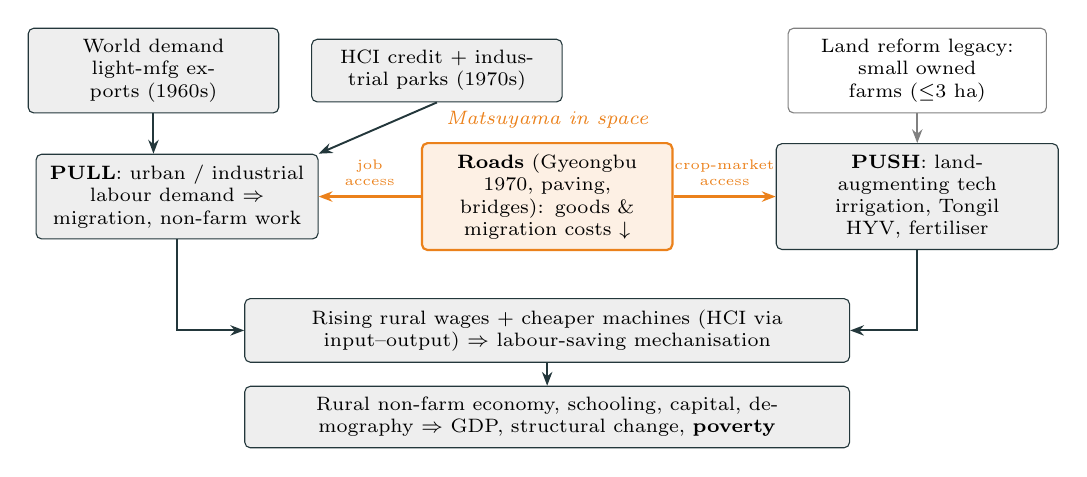
\begin{tikzpicture}
    \node[box=2.9cm] (wd) at (-5.0,0) {World demand\\light-mfg exports (1960s)};
    \node[box=2.9cm] (hci) at (-1.4,0) {HCI credit + industrial parks (1970s)};
    \node[box=3.3cm] (pull) at (-4.7,-1.6)
      {\textbf{PULL}: urban / industrial labour demand $\Rightarrow$ migration, non-farm work};
    \node[box=2.9cm, hot] (roads) at (0,-1.6)
      {\textbf{Roads} (Gyeongbu 1970, paving, bridges): goods \& migration costs $\downarrow$};
    \node[box=3.3cm] (push) at (4.7,-1.6)
      {\textbf{PUSH}: land-augmenting tech\\irrigation, Tongil HYV, fertiliser};
    \node[box=3.0cm, draw=gray, fill=white] (lr) at (4.7,0)
      {Land reform legacy: small owned farms ($\le$3 ha)};
    \node[box=7.4cm] (mech) at (0,-3.3) {Rising rural wages + cheaper machines (HCI
      via input--output) $\Rightarrow$ labour-saving mechanisation};
    \node[box=7.4cm] (agg) at (0,-4.4) {Rural non-farm economy, schooling, capital,
      demography $\Rightarrow$ GDP, structural change, \textbf{poverty}};
    \draw[arr] (wd.south) -- (wd.south |- pull.north);
    \draw[arr] (hci.south) -- (pull.north east);
    \draw[arr, mOrange, line width=1pt] (roads) -- node[above, font=\tiny, text=mOrange,
      align=center] {job\\access} (pull);
    \draw[arr, mOrange, line width=1pt] (roads) -- node[above, font=\tiny, text=mOrange,
      align=center] {crop-market\\access} (push);
    \draw[arr, gray] (lr) -- (push);
    \draw[arr] (pull.south) |- (mech.west);
    \draw[arr] (push.south) |- (mech.east);
    \draw[arr] (mech) -- (agg);
    \node[font=\scriptsize\itshape, text=mOrange, above=0.5mm of roads]
      {Matsuyama in space};
  \end{tikzpicture}
  \vspace{0.3em}

  \small Each arrow needs a model block, a \hl{measured} shock, an \hl{identified}
  elasticity, and a counterfactual that switches it off.
\end{frame}

\begin{frame}{Matsuyama (1992), and why Korea makes it spatial}
  \begin{columns}[T]
    \begin{column}{0.5\textwidth}
      \textbf{Matsuyama (1992, JET)}: manufacturing has learning-by-doing.
      \begin{itemize}\small
        \item \textbf{Closed economy.} Farm productivity $\uparrow$ $\Rightarrow$ food
              needs met with fewer workers (Engel) $\Rightarrow$ labour \hl{released} to
              industry $\Rightarrow$ faster growth. The ``food problem''
              (Gollin--Parente--Rogerson 2007).
        \item \textbf{Open economy.} Farm productivity $\uparrow$ $\Rightarrow$
              comparative advantage in farming $\Rightarrow$ labour \hl{retained}
              $\Rightarrow$ slower industrialisation.
      \end{itemize}
      The Korean narrative implicitly assumes the closed case. Which case applies is
      usually a national question.
    \end{column}
    \begin{column}{0.46\textwidth}
      \begin{alertblock}{Why Korea}
        After 1969 the rice market was \hl{nationally closed and policy-priced} (import
        controls, government procurement under the dual grain-price policy).\\[0.4em]
        A township was \emph{open to the nation} while the nation was \emph{closed to the
        world}.\\[0.4em]
        So the ``regime'' is township-level by construction, and roads move townships
        between regimes.
      \end{alertblock}
    \end{column}
  \end{columns}
\end{frame}

\begin{frame}{The hypothesis, stated carefully}
  \begin{block}{Hypothesis}
    Agricultural productivity growth induces \hl{commercialisation} where access to crop
    demand dominates, and \hl{labour release} where access to non-farm opportunities
    dominates.
  \end{block}
  \footnotesize
  \begin{itemize}
    \item A connectivity-dependent \emph{sign reversal} of the farm-employment response is
          one derivable implication, \textbf{not} the test.
    \item The test: the model, with trade, distance and Engel parameters estimated
          elsewhere, predicts an interaction coefficient $X$; the reservoir event studies
          give $Y$. A \hl{held-out moment}.
    \item Related: Gollin--Rogerson (2014), Sotelo (2020), Foster--Rosenzweig (2004),
          Bustos--Caprettini--Ponticelli (2016).
  \end{itemize}
  \begin{exampleblock}{Novelty}
    \footnotesize
    Cheung--Yang (2024, SSRN 4768158; reportedly JIE, to verify): Indian roads lower
    machine prices relative to wages and induce labour-saving technology. So
    roads $\to$ mechanisation alone will not distinguish us. Our contribution: separately
    identify \emph{farm productivity shocks}, \emph{industrial labour-demand shocks} and
    \emph{connectivity}, and show where their interaction yields commercialisation versus
    release.
  \end{exampleblock}
\end{frame}

% =====================================================================
\section{Core mechanisms}
% =====================================================================

\begin{frame}{A township in one equation}
  Competitive farms, $Q_i=(B_iT_i)^{\alpha}L_{Ai}^{1-\alpha}$; land-augmenting shock $B_i$
  (reservoir). Local crop demand faced with elasticity $e_i$; opportunity wage $w_i$.
  \begin{equation*}
    d\log L_{Ai}
    \;=\;
    \frac{\overbrace{\alpha\,(e_i-1)\,d\log B_i}^{\text{commercialisation vs.\ food problem}}
          \;-\;\overbrace{e_i\,d\log w_i}^{\text{labour release}}}
         {\alpha e_i + 1-\alpha}
  \end{equation*}
  \begin{columns}[T]
    \begin{column}{0.52\textwidth}
      \small
      \begin{itemize}
        \item From the FOC $\log L_A=\tfrac1\alpha[\log p+\alpha\log BT-\log w]+c$ and
              $d\log p=-\tfrac{1}{e}d\log Q$.
        \item \textbf{Goods-market access} raises $e_i$: isolated $\approx$ local food
              elasticity ($<1$); connected $\to\theta$ (4--8).
        \item \textbf{Labour-market access} moves $w_i$ (industrial pull, migration).
        \item Fixed $w$: labour retained iff $e_i>1$.
      \end{itemize}
    \end{column}
    \begin{column}{0.44\textwidth}
      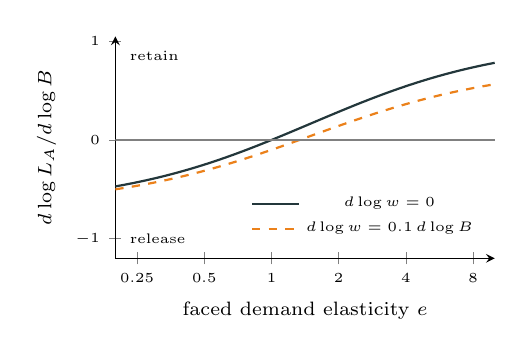
\begin{tikzpicture}
        \begin{axis}[width=6.4cm, height=4.4cm, xmode=log, xmin=0.2, xmax=10,
            ymin=-1.2, ymax=1.05, axis lines=left,
            xlabel={\scriptsize faced demand elasticity $e$},
            ylabel={\scriptsize $d\log L_A/d\log B$},
            tick label style={font=\tiny}, label style={font=\scriptsize},
            xtick={0.25,0.5,1,2,4,8}, xticklabels={0.25,0.5,1,2,4,8},
            legend style={font=\tiny, draw=none, at={(0.98,0.05)}, anchor=south east}]
          \addplot[domain=0.2:10, samples=120, mDarkTeal, thick]
            {0.4*(x-1)/(0.4*x+0.6)};
          \addlegendentry{$d\log w=0$}
          \addplot[domain=0.2:10, samples=120, mOrange, thick, dashed]
            {(0.4*(x-1)-0.1*x)/(0.4*x+0.6)};
          \addlegendentry{$d\log w=0.1\,d\log B$}
          \draw[gray, thin] (axis cs:0.2,0) -- (axis cs:10,0);
          \node[font=\tiny, anchor=north west] at (axis cs:0.21,1.0) {retain};
          \node[font=\tiny, anchor=south west] at (axis cs:0.21,-1.15) {release};
        \end{axis}
      \end{tikzpicture}\\
      \tiny Illustrative, $\alpha=0.4$. Not the quantitative model.
    \end{column}
  \end{columns}
\end{frame}

\begin{frame}{Why the sharp version (``the sign should flip'') is not the test}
  \footnotesize
  \begin{enumerate}
    \item \textbf{Gravity builds in the answer.} Under Armington / EK a connected township
          faces $e=\theta>1$, an isolated one the food elasticity $<1$. The flip holds by
          construction. The data identify \hl{where} on the access distribution the
          crossing occurs, which disciplines distance costs and Engel parameters.
          (Matsuyama's open case also needs a homogeneous traded good; Armington removes it.)
    \item \textbf{Connectivity moves both terms.} Connected townships also have non-farm
          jobs, cheaper machines, lower migration costs: $d\log w>0$ pushes towards release,
          opposite to comparative-advantage retention. A null interaction is
          uninterpretable without separate industrial-pull controls.
    \item \textbf{Irrigation is not Hicks-neutral.} Korean paddy irrigation + Tongil HYV
          raised labour per hectare (double cropping, transplanting). A labour-using shock
          retains labour everywhere. Estimate the factor bias jointly.
  \end{enumerate}
  \begin{alertblock}{Two reconciliations}
    \footnotesize
    (i) \textbf{Rice-price support} from 1969 insulates farm-gate prices from local supply,
    weakening the isolated-township price channel: derive price policy and prediction
    together. (ii) \textbf{Township retention $\neq$ aggregate retardation}: the growth
    conclusion needs manufacturing learning-by-doing.
  \end{alertblock}
\end{frame}

\begin{frame}{Labour-saving technology: mechanisation with an indivisible machine}
  A tiller cuts labour per hectare by a fraction $\chi$ and costs $u_t=p_{m,t}(r_t+d)$ a
  year. A farm of size $\ell$ adopts iff
  \begin{equation*}
    \chi\,\lambda_0\,\ell\,w_{iA,t}\;\ge\;u_t
    \quad\Longleftrightarrow\quad
    \ell\;\ge\;\ell^{*}_{it}=\frac{p_{m,t}\,(r_t+d)}{\chi\,\lambda_0\,w_{iA,t}},
    \qquad
    \text{adoption}_{it}=1-F_i\bigl(\ell^{*}_{it}\bigr).
  \end{equation*}
  \begin{columns}[T]
    \begin{column}{0.55\textwidth}
      \small
      \begin{itemize}
        \item $F_i$ = \hl{observed} landholding distribution (land-reform legacy, 3-ha
              ceiling); custom hiring smooths the threshold.
        \item Adoption responds to local farm wages (\hl{industrial pull}), machine prices
              (\hl{HCI machinery} via input--output) and farm size.
        \item Hayami--Ruttan induced innovation with a micro-founded extensive margin.
      \end{itemize}
    \end{column}
    \begin{column}{0.41\textwidth}
      \begin{block}{The distinction that matters}
        \small
        Labour-saving change \hl{releases} labour; land-augmenting change can
        \hl{absorb} it (Bustos--Caprettini--Ponticelli 2016).\\[0.3em]
        In the current code this margin is a reduced form: a fixed-cost
        mechanised technology with $\xi=1.2$ (next section).
      \end{block}
    \end{column}
  \end{columns}
\end{frame}

\begin{frame}{The agricultural productivity gap needs sectoral wages}
  With one wage per location, farm and non-farm value added per worker differ only through
  labour shares $\lambda^k$:
  \begin{equation*}
    \mathrm{APG}_d\equiv\frac{\mathrm{VA}^A_d/L^A_d}{\mathrm{VA}^N_d/L^N_d}
    =\frac{w^A_d/\lambda^A_d}{w^N_d/\lambda^N_d}
    \;\overset{w^A=w^N}{=}\;\frac{\lambda^N_d}{\lambda^A_d}\;\gtrsim 1 .
  \end{equation*}
  \small
  \begin{itemize}
    \item Land takes a large share of farm VA, so an integrated market delivers APG near
          or above one. The data (0.38 VA / 0.59 employment in 1965\unv) imply
          $\approx 0.43$.
    \item In the calibrated baseline, the 1965 farm VA share is 0.595 against 0.38\unv{} in
          the data: the integrated market cannot open the gap.
    \item Fix: \hl{occupation choice} within location, with a non-pecuniary occupation
          value $b$ (attachment to farming, barriers to leaving it). Gollin--Lagakos--Waugh
          (2014); Hsieh--Hurst--Jones--Klenow (2019).
    \item Policy content: if roads and schooling lower the farm wedge, that is a
          mechanism of structural change in its own right, and the decomposition prices it.
  \end{itemize}
\end{frame}

% =====================================================================
\section{Theory: the current model}
% =====================================================================

\begin{frame}{Environment}
  \begin{columns}[T]
    \begin{column}{0.5\textwidth}
      \small
      \textbf{Sequence of static spatial equilibria}, state $=L_{t-1}$.\\[0.3em]
      \begin{itemize}
        \item Locations $d\in\mathcal N$ (5 stylised: Seoul, Busan, Changwon, Daegu,
              Rural); periods 1965/68/73/75/80/85.
        \item \textbf{Sectors}:
          \begin{itemize}\footnotesize
            \item \textbf{Rice}: protected, internationally non-traded; carries the
                  mechanisation margin.
            \item \textbf{OtherAg}: import-competing at world prices; not exported.
            \item \textbf{Manufacturing}: traded; the export sector.
            \item \textbf{Services}: non-traded.
          \end{itemize}
        \item Input--output linkages; sector-specific agglomeration $L_{o,t-1}^{\rho_j}$.
      \end{itemize}
    \end{column}
    \begin{column}{0.46\textwidth}
      \small
      \begin{itemize}
        \item PIGL non-homothetic demand (Boppart 2014).
        \item Gumbel migration (myopic), now \hl{nested} with occupation choice.
        \item Monopolistic competition with bounded Pareto draws; \hl{nested}
              entry / adoption / export choice.
        \item Local land ownership; nationally pooled profits; government buys output.
        \item Small open economy; numeraire: foreign manufacturing price;
              net exports \hl{pinned exogenously}.
        \item Growth engine: sectoral TFP growth + rising foreign demand for manufactures.
      \end{itemize}
    \end{column}
  \end{columns}
\end{frame}

\begin{frame}{Preferences: PIGL and the food problem}
  Indirect utility and expenditure shares at income $y$, prices $P_{dj}$,
  $\mathcal P_d=\prod_jP_{dj}^{\alpha_j}$:
  \begin{equation*}
    V_d=\frac1\eta\Bigl(\frac{y}{\mathcal P_d}\Bigr)^{\eta}-\sum_j v_j\log P_{dj},
    \qquad
    \psi_{dj}=\alpha_j+v_j\Bigl(\frac{y}{\mathcal P_d}\Bigr)^{-\eta},
    \qquad \textstyle\sum_j\alpha_j=1,\ \sum_jv_j=0.
  \end{equation*}
  \small
  \begin{itemize}
    \item $\eta>0$, $v_{\text{food}}>0$: the food share falls with real income (Engel),
          services rise. Calibrated $\eta=0.39$.
    \item Shares checked in $[0,1]$ along the solved path, not just imposed.
    \item Exact aggregation over finitely many income groups, so farm/non-farm income
          differences change the \emph{composition} of local demand.
    \item Migration and welfare use the \hl{exact equivalent income}
          $\mathcal Y=\mathcal P_0[\eta(V+z_0)]^{1/\eta}$, a monotone transform of $V$
          for every $\eta$. (The old index $x e^{-z}$ was not, and had the wrong income
          elasticity.)
    \item Limitation: Cobb--Douglas price aggregator, so no Baumol relative-price channel.
          Non-homothetic CES (Comin--Lashkari--Mestieri) if the data call for it.
  \end{itemize}
\end{frame}

\begin{frame}{Location $\times$ occupation choice}
  Agent in origin $o$ chooses location $d$ and occupation $\kappa\in\{$farm, mfg,
  services$\}$ to maximise
  $W_{od}+\log b_{d\kappa}+\log\mathcal Y_{d\kappa}+\upsilon_{i,d\kappa}$, with GEV shocks
  $G(x)=\sum_d\bigl(\sum_\kappa x_{d\kappa}^{\varepsilon}\bigr)^{\nu/\varepsilon}$:
  \begin{equation*}
    \pi_{\kappa\mid d}=\frac{(b_{d\kappa}\mathcal Y_{d\kappa})^{\varepsilon}}
                            {\sum_{\kappa'}(b_{d\kappa'}\mathcal Y_{d\kappa'})^{\varepsilon}},
    \qquad
    \Phi_d=\Bigl[\sum_\kappa(b_{d\kappa}\mathcal Y_{d\kappa})^{\varepsilon}\Bigr]^{1/\varepsilon},
    \qquad
    \mu_{od}\propto\Bigl(\frac{\bar V_d\,L_{d,t-1}^{\iota}\,\Phi_d}{\delta_{od}}\Bigr)^{\nu}.
  \end{equation*}
  \small
  \begin{itemize}
    \item Random-utility consistent iff $\nu\le\varepsilon$: switching sector within a
          location is easier than moving.
    \item Each location--occupation labour market clears at its own wage
          $w_{d\kappa}L_{d\kappa}=\sum_{j:o(j)=\kappa}[\text{labour share of }TFC_{dj}+\text{fixed-cost bill}]$.
    \item Rice and other crops are \emph{one} occupation: they are products, not labour
          markets (two would double farming's taste mass).
    \item Welfare: $\partial\,\mathbb E U_o/\partial\log\mathcal Y_{d\kappa}=\mu_{od}\pi_{\kappa\mid d}$ (tested).
    \item Integrated limit: $\varepsilon\to\infty$, $b=1$ gives one wage per location.
  \end{itemize}
\end{frame}

\begin{frame}{What the occupation block buys}
  \begin{block}{Wage-gap decomposition (exact in equivalent incomes)}
    \vspace{-0.6em}
    \begin{equation*}
      \log\frac{\mathcal Y_{dA}}{\mathcal Y_{dN}}
      =\underbrace{\frac1\varepsilon\log\frac{L_{dA}}{L_{dN}}}_{\text{supply term}}
      \;-\;\underbrace{\log\frac{b_{dA}}{b_{dN}}}_{\text{non-pecuniary wedge}}
    \end{equation*}
  \end{block}
  \small
  \begin{enumerate}
    \item \textbf{$b=1$ is not frictionless.} It means equal pay $\Rightarrow$ equal
          occupation shares. A 60\% farm share at a \emph{lower} farm wage needs
          $b_A>b_N$.
    \item \textbf{The gap moves with structural change.} When farm labour demand falls
          (Engel, import competition, mechanisation), finite $\varepsilon$ keeps workers
          in farming at a falling relative wage: the gap \hl{widens} before switching and
          migration catch up.
    \item \textbf{Sectoral labour supply:}
          $\partial\log L_{d\kappa}/\partial\log y_{d\kappa}=\varepsilon(1-\pi_{\kappa\mid d})\,e^{\mathcal Y}_{d\kappa}$.
    \item \textbf{Taste vs.\ selection.} A Roy/Fr\'echet version (Lagakos--Waugh 2013)
          is a tractable extension, and predicts different earnings changes for switchers
          (Hamory et al.\ 2021).
  \end{enumerate}
\end{frame}

\begin{frame}{Production: nested entry, adoption and export}
  \small
  With $x=\phi^{\sigma-1}$, every option's profit is linear in $x$: option $k$ has slope
  $a_k$ and fixed cost $c_k$. Agriculture: exit $(0,0)$, traditional $(a^T,F)$, mechanised
  $(a^M,F+\breve F)$, mechanised exporter $(a^M+a^X,F+\breve F+\tilde F)$. The firm picks
  the upper envelope:
  \begin{equation*}
    \text{``option }k\text{ or higher''}\iff x\ge X_k,\qquad
    X_k=\min_{k'\ge k}\;\max_{i<k'}\frac{c_{k'}-c_i}{a_{k'}-a_i}.
  \end{equation*}
  Ordering $\bar\phi\le\breve\phi\le\tilde\phi$ holds by construction; adopters and
  exporters are active firms. A traditional segment exists iff
  \begin{equation*}
    \frac{\breve F}{F}>\Delta,\qquad
    \frac{\breve F+\tilde F}{F}>\Delta+\frac{a^X}{a^T},\qquad
    \Delta\equiv\Bigl(\xi\,\frac{c}{\breve c}\Bigr)^{\sigma-1}-1 .
  \end{equation*}
  \begin{itemize}
    \item $\Delta$ rises with $w/P_{\text{mfg}}$: the mechanised technology substitutes
          machinery for labour, so adoption turns on as \hl{wages rise and machines get
          cheaper} (induced innovation). Hence $\xi=1.2\approx$ the 1965--85 range of
          $\breve c/c$; fixed costs are in labour units.
    \item The old pairwise cutoffs had $\tilde\phi<\breve\phi<\bar\phi$: farms exported and
          mechanised without entering.
  \end{itemize}
\end{frame}

\begin{frame}{External balance pins the wage level}
  \begin{columns}[T]
    \begin{column}{0.5\textwidth}
      \small
      \textbf{The old closure} set the foreign transfer $T=\mathrm{IM}-\mathrm{EX}$ at the
      current guess. Household budgets + goods-market clearing already imply this at any
      fixed point, so one equation was lost.\\[0.4em]
      One-good example: $d(w)E+X(w)=wL$ and $E=wL+T$ with $T=(1-d)E-X$ are the same
      equation $\Rightarrow$ every $w$ solves.\\[0.4em]
      \textbf{Fix}: $\mathrm{EX}-\mathrm{IM}=\mathrm{NX}^\star$ exogenous (default 0;
      later the observed path, deficits financing investment). The domestic price level
      clears the foreign account. Guess-invariant to $3\times10^{-13}$.
    \end{column}
    \begin{column}{0.46\textwidth}
      \footnotesize
      \begin{tabular}{@{}lccc@{}}
        \toprule
        guess $\times k$ & 0.5 & 1.0 & 2.0 \\
        \midrule
        $w_{\text{Seoul}}$ & 0.291 & 0.367 & 0.480 \\
        $(\mathrm{EX}-\mathrm{IM})/\text{abs.}$ & $-0.37$ & $-0.56$ & $-0.67$ \\
        mean real income & 0.96 & 1.92 & 3.50 \\
        \bottomrule
      \end{tabular}\\[0.2em]
      \tiny Old closure, residuals $<10^{-11}$ in every column.\\[0.6em]
      \small
      \textbf{Consequence}: the aggregate export elasticity $\sigma_x$ (separate from
      $\sigma$) now does real work. Old 3-sector HCI headline, 1985 heavy-mfg
      gross-output share effect:\\[0.2em]
      \footnotesize
      \begin{tabular}{@{}lccc@{}}
        \toprule
        $\sigma_x$ & 2 & 4 & 6 \\
        \midrule
        effect & $+0.021$ & $+0.103$ & $+0.137$ \\
        \bottomrule
      \end{tabular}
    \end{column}
  \end{columns}
\end{frame}

\begin{frame}{Equilibrium and solution}
  \small
  Given $L_{t-1}$ and period-$t$ fundamentals, an equilibrium is
  $\{w_{d\kappa},r_d,P_{dj},E_{dj},L_d,\bar\tau,\bar\pi\}$ such that:
  \begin{enumerate}
    \item \textbf{Migration and occupation}: $\mu_{od}$, $\pi_{\kappa\mid d}$ as above;
          $L_d=\sum_o\mu_{od}L_{o,t-1}$, $L_{d\kappa}=\pi_{\kappa\mid d}L_d$.
    \item \textbf{Final demand}: PIGL shares summed over occupation income groups.
    \item \textbf{Firms}: nested cutoffs, productivity aggregates, price indices, revenues.
    \item \textbf{Expenditure}: $E=E^F+E^M+E^G$; intermediates from true factor cost
          $TFC=\frac{\sigma-1}{\sigma(1-s)}Y$.
    \item \textbf{Factor markets}: each location--occupation labour market and each land
          market clears; fixed costs are paid to local labour.
    \item \textbf{Government}: $\bar\tau$ finances subsidies and infrastructure (which buys
          goods); $\bar\pi$ rebates pooled profits (sign-unrestricted).
    \item \textbf{External balance}: $\mathrm{EX}-\mathrm{IM}=\mathrm{NX}^\star$.
  \end{enumerate}
  Damped fixed point in $(w,r,P,E,\bar\tau,\bar\pi)$; relative occupation wages by a
  log-Newton step $\Delta\log w_{d\kappa}=\log(D_{d\kappa}/S_{d\kappa})/(1+\varepsilon)$.
  Walras, resource and budget identities hold to $\sim10^{-13}$ (tested).\\[0.3em]
  \textbf{Amenity inversion}: with $L_{1965}$ pinned, the rest of the equilibrium does not
  depend on $\bar V$, so $\bar V$ is recovered exactly from the logit. The observed 1965
  population is an equilibrium; later urbanisation is a \hl{model outcome}.
\end{frame}

\begin{frame}{Where the model is heading: five principles}
  \scriptsize
  \begin{tabular}{@{}L{0.2\textwidth}L{0.5\textwidth}L{0.24\textwidth}@{}}
    \toprule
    Principle & Content & Replaces \\
    \midrule
    1. Baseline = history &
      Annual 1962--90; invert fundamentals each year (once identified); programmes as
      measured shocks; Shapley decomposition &
      Hand-set paths; 6 uneven periods; policy $-$ baseline \\
    2. Simplify production &
      CES gravity (Armington/EK) with sectoral external economies in employment density &
      Melitz everywhere \\
    3. People in sectors &
      Nested location $\times$ occupation incl.\ non-employment (Lewis surplus labour) &
      Single regional wage \\
    4. Agriculture on observed land &
      Competitive farm households on paddy and dry fields; farm-size classes; irrigation,
      HYV; mechanisation threshold in $w/p_m$ &
      Monopolistic ``farms'' with fixed adoption cost \\
    5. Growth engines &
      Capital with HCI credit wedges and foreign saving; schooling; demography; world
      demand; poverty and welfare as outputs &
      Output subsidies; fixed population \\
    \bottomrule
  \end{tabular}
  \vspace{0.4em}
  \begin{equation*}
    \pi_{in,k}=\frac{(\tau_{in,k}c_{ik}/A_{ik})^{-\theta_k}}
      {\sum_l(\tau_{ln,k}c_{lk}/A_{lk})^{-\theta_k}+(\tilde\tau_{n,k}\tilde p_k)^{-\theta_k}},
    \qquad
    A_{ik}=\bar A_{ik}\Bigl(\frac{L_{ik}}{\text{area}_i}\Bigr)^{\rho_k},
    \qquad
    \tau_{in,k}=e^{\varphi_k\,\text{time}_{in}}\,a_ia_n .
  \end{equation*}
  \centering\scriptsize Done so far: (3) without non-employment; (4) only as Rice/OtherAg
  split; (5) only TFP + world demand.
\end{frame}

\begin{frame}{The annual inversion is not identified as written}
  \small
  Per township--year under principles 2--3:
  \begin{center}
    \begin{tabular}{@{}lll@{}}
      \toprule
      Unknowns & $K$ productivities $+$ $(K-1)$ wedges $+$ 1 amenity & $=2K$ \\
      Observables & population $+$ $(K-1)$ employment shares & $=K$ \\
      \bottomrule
    \end{tabular}
  \end{center}
  In $\pi_{k\mid i}\propto(b_{ik}w_{ik})^{\varepsilon}$, higher $A_{ik}$ raises $w_{ik}$
  and hence $\pi_{k\mid i}$ \emph{exactly} as higher $b_{ik}$ does.
  \begin{itemize}
    \item Need wages, output, prices or trade flows: county MMS wages and VA, provincial
          farm wages, crop output and prices. Or restrictions: wedges common within
          county/province, or constant up to trend.
    \item Demonstrate identification (analytically or by recovery on synthetic data)
          \hl{before} building \texttt{inversion.py} beyond amenities.
    \item Inverted fundamentals are not causal policy effects: event studies on them need
          the same assignment design and must carry inversion uncertainty.
    \item Exact fit is not validation: inversion inputs cannot also validate.
  \end{itemize}
\end{frame}

% =====================================================================
\section{Calibration and data}
% =====================================================================

\begin{frame}{History calibration: 8 parameters, 8 targets}
  \begin{columns}[T]
    \begin{column}{0.6\textwidth}
      \scriptsize
      \begin{tabular}{@{}lll@{}}
        \toprule
        Parameter & Value & Main target \\
        \midrule
        $g_{\text{mfg}}$ (TFP growth) & 4.1\%/yr & real GDP p.c.\ 1985/65 \\
        $g_{\text{farm}}=g_{\text{svc}}$ & 3.2\%/yr & mfg VA share 1985 \\
        $\eta$ (PIGL) & 0.39 & farm emp.\ share 1985 \\
        $v_{\text{food}}$ (Engel shifter) & 0.51 & farm emp.\ share 1965 \\
        mfg share of non-food $\alpha$ & 0.02 (bound) & mfg VA share 1965 \\
        foreign demand, 1965 level & 0.0044 & exports/GDP 1965 \\
        foreign demand growth & 24\%/yr & exports/GDP 1985 \\
        urban non-farm TFP premium & 1.17 & urban share 1980 \\
        \bottomrule
      \end{tabular}\\[0.3em]
      \tiny \texttt{scripts/calibrate\_history.py}: least squares; each evaluation first
      inverts 1965 amenities; PIGL share bounds as a penalty.
    \end{column}
    \begin{column}{0.36\textwidth}
      \footnotesize
      \textbf{Held fixed} (from earlier calibration or assumption): $\sigma=4$,
      $\theta=5$, $\nu=5$, $\xi=1.2$, $\rho_j$, IO coefficients, land shares, trade and
      migration cost matrices.\\[0.4em]
      \textbf{Assumed, no data yet}:
      \begin{itemize}\footnotesize
        \item rice = half of food demand
        \item urban farm TFP = 0.4 $\times$ rural
        \item food asymptote $\alpha_{\text{food}}=0.05$
        \item 1965 city split stylised
        \item rice mechanisation fixed cost
        \item services TFP growth = farm
      \end{itemize}
    \end{column}
  \end{columns}
\end{frame}

\begin{frame}{The baseline reproduces the 1965--85 transformation}
  \centering
  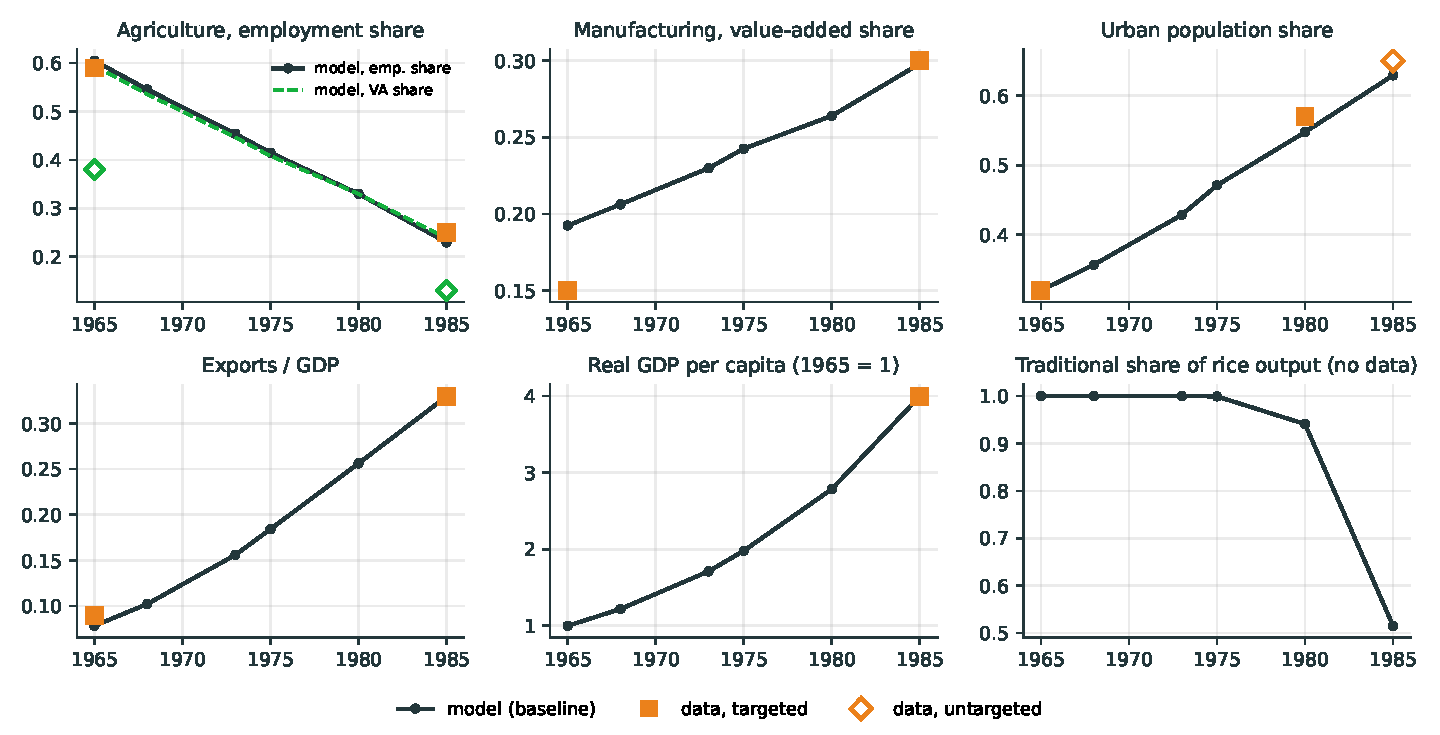
\includegraphics[width=0.94\textwidth]{fig_history_fit.pdf}\\
  \scriptsize Solved at the current calibration (\texttt{make\_figures.py}). Green: farm
  value-added share (model, dashed; data, hollow).
\end{frame}

\begin{frame}{Fit, and what it establishes}
  \begin{columns}[T]
    \begin{column}{0.52\textwidth}
      \footnotesize
      \begin{tabular}{@{}lccl@{}}
        \toprule
        1965 $\to$ 1985 & data & model & \\
        \midrule
        farm emp.\ share & .59\unv{}$\to$.25\unv & .605$\to$.229 & T \\
        mfg VA share & .15$\to$.30 & .192$\to$.298 & T \\
        real GDP p.c. & $\times$4\unv & $\times$4.00 & T \\
        exports / GDP & .09\unv{}$\to$.33\unv & .078$\to$.330 & T \\
        urban share 1980 & .57 & .547 & T \\
        urban share 1985 & .65\unv & .629 & U \\
        farm VA share & .38\unv{}$\to$.13\unv & .595$\to$.239 & U \\
        OtherAg import share & --- & .095$\to$.764 & \\
        trad.\ rice share & $\sim$1$\to$$<$1 & 1.00$\to$.515 & \\
        \bottomrule
      \end{tabular}\\[0.2em]
      \tiny T targeted, U untargeted. Guess-invariant to $5\times10^{-12}$.
    \end{column}
    \begin{column}{0.44\textwidth}
      \small
      \begin{itemize}
        \item Farm employment falls 38 points through \hl{Engel effects} on rising
              income, \hl{grain import competition}, and \hl{migration}, while the economy
              grows fourfold and urbanises from 0.32 to 0.63.
        \item Exports 8\% $\to$ 33\% of GDP requires foreign demand growing 24\%/yr at
              $\sigma=4$.
        \item Rice mechanisation takes off only after 1975, as wages rise: the
              induced-innovation timing, but its level is set by an assumed fixed cost.
      \end{itemize}
    \end{column}
  \end{columns}
\end{frame}

\begin{frame}{Mechanical limits of the current baseline}
  \small
  \begin{enumerate}
    \item \textbf{No agricultural productivity gap.} Rural wage 0.76 of urban in 1965;
          farm VA share 0.595 vs 0.38\unv. Matching it with one wage per region would need
          a rural/urban wage ratio of $\sim$1/3. $\Rightarrow$ occupation block (next
          slide), not yet recalibrated.
    \item \textbf{1965 manufacturing share too high} (0.19 vs 0.15) with the final-demand
          weight at its lower bound: the stylised IO coefficients over-produce
          manufacturing. $\Rightarrow$ BoK input--output tables.
    \item \textbf{No relative-price channel} in demand: farm TFP releases labour only
          through income and import competition, not Baumol.
  \end{enumerate}
  \begin{alertblock}{HCI under this baseline: unresolved, not a finding}
    The (untuned) HCI package \emph{lowers} the 1985 national manufacturing share (VA
    $-0.013$, employment $-0.026$) and raises services. The sign comes from the baseline,
    not one channel: income gains go to non-traded services, and manufacturing has almost
    no domestic final demand (limit 2). The directional test is a strict expected failure
    until the IO structure comes from data.
  \end{alertblock}
\end{frame}

\begin{frame}{Occupation choice in the Korea baseline (illustration, not recalibrated)}
  \footnotesize
  \centering
  \begin{tabular}{@{}lcccccc@{}}
    \toprule
    & \multicolumn{3}{c}{1965} & \multicolumn{3}{c}{1985} \\
    \cmidrule(lr){2-4}\cmidrule(lr){5-7}
    case & farm emp. & $w_A/w_N$ & APG & farm emp. & $w_A/w_N$ & APG \\
    \midrule
    integrated ($\varepsilon=\infty$) & 0.605 & 0.827 & 0.958 & 0.229 & 0.868 & 1.053 \\
    $\varepsilon=10$, $b_A=1$ & 0.561 & 0.951 & 1.100 & 0.219 & 0.905 & 1.103 \\
    $\varepsilon=5$, $b_A=1$ & 0.530 & 1.051 & 1.214 & 0.218 & 0.908 & 1.107 \\
    $\varepsilon=5$, $b_A=1.5$ & 0.627 & 0.802 & 0.930 & 0.314 & 0.676 & 0.803 \\
    $\varepsilon=5$, $b_A=2$ & 0.680 & 0.653 & \hl{0.758} & 0.399 & 0.545 & \hl{0.638} \\
    \bottomrule
  \end{tabular}\\[0.2em]
  \tiny 1965 amenities re-inverted per case; all other parameters at the integrated
  calibration. Wage ratios national, employment-weighted. APG = farm VA per worker / non-farm.
  \vspace{0.4em}
  \begin{enumerate}\small
    \item $b_A=1$ makes things \emph{worse}: a large farm share then needs a higher farm wage.
    \item With a farm wedge the gap \hl{appears and widens} during the transformation
          ($b_A=2$: APG 0.76 $\to$ 0.64). The integrated model cannot do this.
    \item The wedge also \hl{slows} the transformation (farm emp.\ 0.40 vs 0.23 in 1985).
          Recalibration trades $(b_A,\varepsilon)$ off against the Engel parameters;
          separating them needs farm vs non-farm earnings data.
  \end{enumerate}
\end{frame}

\begin{frame}{What the township panel does inside the model}
  \footnotesize
  \scriptsize
  \begin{tabular}{@{}L{0.24\textwidth}L{0.46\textwidth}L{0.24\textwidth}@{}}
    \toprule
    Variable & Model object & Role \\
    \midrule
    Population; status & $L_{i,t}$ (amenities); non-employment share & Inversion, estimation \\
    Employment by sector & $\pi_{k\mid n}$; $A_{ik}$, $b_{nk}$ & I, E, V (Fig.\ 8 gradient) \\
    Land (paddy/dry); farm-size classes & land endowments; $F_i(\ell)$ & I (mechanisation threshold) \\
    Reservoirs (capacity, date) & irrigation shock to paddy quality & \hl{Shock}; event studies \\
    Crops, livestock, stores & crop mix, yields, commercialisation & E (von Th\"unen), V \\
    Municipal finance & local public investment by function; transfers & Shock \\
    Roads paved/unpaved, bridges & local access $a_{i,t}$; annual paving dates & \hl{Shock} \\
    Electricity; schools & non-farm productivity; cohort human capital & Shock, I, E \\
    \bottomrule
  \end{tabular}\\[0.3em]
  \tiny I = inversion input; E = estimation moment; V = held-out validation.\\[0.4em]
  \small
  \textbf{Identification map}: $\theta,\varphi$ from price gaps (Donaldson) or indirect
  inference on market-access event studies; $\nu,\delta$ from O--D gravity and interchange
  openings; $\varepsilon,b$ from shift-share industrial pull; $\rho_k$ from park SDID and
  the post-1979 wind-down; $\eta,v_j$ from household-survey Engel curves; mechanisation
  from adoption by farm-size class $\times$ wage and machine-price shocks.
\end{frame}

\begin{frame}{The reservoir design: the empirical side of Matsuyama in space}
  \small
  \begin{columns}[T]
    \begin{column}{0.5\textwidth}
      \begin{itemize}
        \item Event studies of reservoir completions, heterogeneous by \hl{predetermined}
              access to \emph{crop markets} and, \hl{separately}, to \emph{non-farm
              employment}.
        \item Treatment: irrigation \emph{command area} and water delivery, not the
              township containing the dam. Handle construction jobs, roads,
              displacement, downstream effects.
        \item Placebo: dry-field townships.
        \item Use the farm employment \emph{share} (migration contaminates levels).
        \item A positive interaction is not a reversal: show the irrigation effect
              \hl{crosses zero} within the observed support.
      \end{itemize}
    \end{column}
    \begin{column}{0.46\textwidth}
      \footnotesize
      \begin{tabular}{@{}L{0.3\textwidth}L{0.62\textwidth}@{}}
        \toprule
        Channel & Evidence \\
        \midrule
        Commercia\-lisation & marketed output, farm-gate prices, farm labour demand,
          land returns \\
        Labour release & labour per hectare $\downarrow$, mechanisation, non-farm work,
          migration \\
        Local demand spillovers & rural services employment after farm-income gains \\
        \bottomrule
      \end{tabular}\\[0.4em]
      \small Model side: derive the predicted coefficients with $\theta,\varphi,\eta$ set
      elsewhere, then compare (indirect inference).
    \end{column}
  \end{columns}
\end{frame}

\begin{frame}{Build order}
  \footnotesize
  \begin{tabular}{@{}lL{0.58\textwidth}L{0.3\textwidth}@{}}
    \toprule
    Stage & Content & Deliverable \\
    \midrule
    0 (done) & Closure, measurement, nested choice, $\sigma_x$, equivalent income;
      history baseline; occupation block &
      Numbers that measure what their labels say \\
    \textbf{1} & \textbf{Small spatial agriculture model}: paddy/dry, competitive farms,
      factor-biased irrigation, non-farm sector, land, trade, mobility &
      Commercialisation-vs-release prediction \\
    \textbf{2} & \textbf{Reservoir event studies} (command areas, separate access measures) &
      Empirical side, standalone \\
    3 & Annual clock, gravity, inversion (after identification), occupation with
      non-employment, structural event studies & Where and when fundamentals moved \\
    4 & Capital, schooling, demography, poverty; Shapley decomposition & The macro paper \\
    \bottomrule
  \end{tabular}
  \par\vspace{1em}
  \small Stages 1--2 come first because they test the mechanism behind ``Matsuyama in
  space'' before a large model exists. Annual timing, competitive agriculture and a simpler
  trade block are sensible from Stage 1.
\end{frame}

\begin{frame}{Decisions for us}
  \small
  \begin{block}{To agree on \mute{\normalfont\scriptsize(recommendations from \texttt{fresh\_look.md} \S9)}}
    \begin{enumerate}
      \item Adopt ``baseline = history + decomposition'' with poverty and structural
            transformation as headline outcomes? \mute{(recommended)}
      \item Drop Melitz in the macro model; keep firm heterogeneity for an MMS satellite?
            \mute{(recommended)}
      \item Capital: observed aggregate investment first, endogenous saving later?
            \mute{(recommended)}
      \item Geography: townships + urban units, counties for manufacturing? Needs urban
            coverage confirmed; consider commuting zones (township data are by residence).
      \item Closure data: feed the observed NX/GDP path once the model is annual?
            \mute{(recommended)}
    \end{enumerate}
  \end{block}
  \begin{alertblock}{And the near-term modelling calls}
    \begin{itemize}
      \item Recalibrate with the occupation block on, once farm/non-farm earnings are in.
      \item Replace stylised IO coefficients with BoK tables before reading any HCI number.
      \item Calibrate $\sigma_x$ externally; report headlines with its sensitivity.
    \end{itemize}
  \end{alertblock}
\end{frame}

\begin{frame}{Data we most need (cheap now, expensive after the freeze)}
  \begin{columns}[T]
    \begin{column}{0.5\textwidth}
      \textbf{To recalibrate the current model}
      \begin{itemize}\footnotesize
        \item Farm vs non-farm earnings (APG; separates $b_A$, $\varepsilon$, Engel)
        \item Food expenditure share by income (PIGL directly)
        \item Grain self-sufficiency / import shares
        \item Rice's share of food spending
        \item Power tillers per farm household, 1965--85
        \item Sectoral productivity growth (GGDC 10-sector)
        \item BoK input--output tables
        \item Regional population and farm employment
        \item Verify every \unv{} target against source
      \end{itemize}
    \end{column}
    \begin{column}{0.46\textwidth}
      \textbf{Asks for the digitisation team}
      \begin{itemize}\footnotesize
        \item Urban units (dong/gu/si): the destination side of every flow
        \item Annual boundary crosswalk with area weights
        \item Variable-year metadata; double-entry sample
        \item Local prices: rice, barley, fertiliser, tillers, farm wages
        \item Irrigated vs rain-fed paddy; output by crop and \hl{rice variety} (Tongil);
              machinery stocks; landholding classes in full
        \item Population by age and sex; births and deaths
        \item Municipal finance chart of accounts; schools entrants/graduates
      \end{itemize}
    \end{column}
  \end{columns}
\end{frame}

\begin{frame}[standout]
  Farm productivity growth: \\ commercialisation or labour release?\\[0.5em]
  \normalsize It depends on where you are.\\
  Korea lets us measure where.
\end{frame}

% =====================================================================
\appendix
\metroset{sectionpage=none}
\section{Backup}
% =====================================================================

\begin{frame}{Backup: how the old HCI headline moved}
  \footnotesize
  \centering
  \begin{tabular}{@{}lcccc@{}}
    \toprule
    1985, policy $-$ baseline (old 3-sector economy) & old closure & determinate & + nested & + ag recal.\ \\
    \midrule
    heavy-mfg gross-output share & $+0.057$ & $+0.104$ & $+0.095$ & $+0.103$ \\
    agriculture share & $-0.041$ & $-0.045$ & $-0.040$ & $-0.005$ \\
    services share & $-0.016$ & $-0.060$ & $-0.055$ & $-0.098$ \\
    Changwon wage & $+0.144$ & $+0.120$ & $+0.122$ & $+0.087$ \\
    rural income per capita & $+0.199$ & $+0.171$ & $+0.174$ & $+0.121$ \\
    \bottomrule
  \end{tabular}
  \vspace{0.5em}
  \begin{itemize}\small
    \item Pre-accounting-fix code (\texttt{cdafe29}) gave $+0.127$ and was determinate. Old
          accounts $\to$ corrected accounts with balanced trade: $+0.127\to+0.104$. The
          further fall to $+0.057$ was the indeterminate closure's selection.
    \item All of this is superseded by the history-calibrated 4-sector baseline, under
          which the HCI aggregate effect is unresolved.
  \end{itemize}
\end{frame}

\begin{frame}{Backup: counterfactuals that tell the story}
  \small
  \begin{enumerate}
    \item \textbf{Decomposition of 1962--90 growth and poverty reduction} over drivers
          $D=\{$world demand, capital, human capital, demography, HCI credit, parks, roads,
          rural programmes, residual TFP$\}$:
          \begin{equation*}
            \phi_d=\sum_{S\subseteq D\setminus\{d\}}\frac{|S|!\,(|D|-|S|-1)!}{|D|!}\,
            \bigl[Y(S\cup\{d\})-Y(S)\bigr].
          \end{equation*}
          10 drivers $=1{,}024$ dynamic solves; 5 blocks $=32$.
    \item \textbf{Complementarity}: $Y(a,b)-Y(a)-Y(b)+Y(\varnothing)$ for parks $\times$
          roads, roads $\times$ rural programmes, schooling $\times$ HCI.
    \item \textbf{Sequencing}: roads before parks; Green Revolution before mechanisation.
    \item \textbf{Incidence}: who escaped poverty, by origin-township type and land class.
    \item \textbf{Persistence / big push}: remove HCI wedges after 1979.
  \end{enumerate}
  Poverty headcount from cell incomes with lognormal dispersion:
  $H_t=\sum_c\omega_{c,t}\,\Phi\bigl(\frac{\ln z-\ln\bar y_{c,t}}{\sigma_c}+\frac{\sigma_c}{2}\bigr)$.
\end{frame}

\begin{frame}{Backup: derivation of the township equation}
  \small
  Competitive farm, Cobb--Douglas: $p(1-\alpha)Q/L_A=w$ with $Q=(BT)^\alpha L_A^{1-\alpha}$
  gives
  \begin{equation*}
    \log L_A=\tfrac1\alpha\bigl[\log(1-\alpha)+\log p+\alpha\log(BT)-\log w\bigr].
  \end{equation*}
  Faced demand $Q=D\,p^{-e}$, so $d\log p=-\frac1e\,d\log Q=-\frac1e[\alpha\,d\log B+(1-\alpha)\,d\log L_A]$.
  Substituting and collecting $d\log L_A$:
  \begin{equation*}
    d\log L_A\Bigl(\alpha+\frac{1-\alpha}{e}\Bigr)=\alpha\Bigl(1-\frac1e\Bigr)d\log B-d\log w
    \;\Longrightarrow\;
    d\log L_A=\frac{\alpha(e-1)\,d\log B-e\,d\log w}{\alpha e+1-\alpha}.
  \end{equation*}
  \begin{itemize}
    \item $e\to\infty$ (price-taker): $d\log L_A=d\log B-\frac1\alpha d\log w$, the
          general form in the referee report.
    \item Note the release term is \emph{larger} where $e$ is large: connected townships
          respond more to the opportunity wage as well.
    \item Partial equilibrium and Hicks-neutral; the quantitative model replaces both.
  \end{itemize}
\end{frame}

\begin{frame}{References}
  \begin{columns}[T]
    \begin{column}{0.48\textwidth}
    \scriptsize
    \begin{itemize}\setlength{\itemsep}{0pt}
      \item Adão, Arkolakis \& Esposito (2019) General equilibrium effects in space
      \item Allen \& Arkolakis (2014, QJE)
      \item Boppart (2014, ECMA)
      \item Budí-Ors \& Pijoan-Mas (WP) Rural exodus and uneven industrialisation
      \item Buera, Kaboski \& Townsend (2023, JEL)
      \item Bustos, Caprettini \& Ponticelli (2016, AER)
      \item Caliendo, Dvorkin \& Parro (2019, ECMA)
      \item Cheung \& Yang (2024, SSRN 4768158) Transportation networks, technology adoption, and structural transformation
      \item Comin, Lashkari \& Mestieri (2021, ECMA)
      \item Dekle, Eaton \& Kortum (2008)
      \item Donaldson (2018, AER)
      \item Eckert \& Peters (WP) Spatial structural change
      \item Fan, Peters \& Zilibotti (2023, ECMA)
      \item Foster \& Rosenzweig (2004, EDCC)
      \item Gollin, Lagakos \& Waugh (2014, QJE)
      \item Gollin, Parente \& Rogerson (2007, JME)
      \item Gollin \& Rogerson (2014, JDE)
    \end{itemize}
    \end{column}
    \begin{column}{0.48\textwidth}
    \scriptsize
    \begin{itemize}\setlength{\itemsep}{0pt}
      \item Hamory, Kleemans, Li \& Miguel (2021, JEEA)
      \item Hayami \& Ruttan (1971)
      \item Hsieh, Hurst, Jones \& Klenow (2019, ECMA)
      \item Kleinman, Liu \& Redding (2023, ECMA)
      \item Kucheryavyy, Lyn \& Rodríguez-Clare (2023, AEJ:Macro)
      \item Lagakos \& Waugh (2013, AER)
      \item Lagakos, Mobarak \& Waugh (2023, ECMA)
      \item Lewis (1954)
      \item Matsuyama (1992, JET) Agricultural productivity, comparative advantage, and economic growth
      \item McFadden (1978)
      \item Nakamura \& Steinsson (2018, JEP)
      \item Redding \& Rossi-Hansberg (2017, ARE)
      \item Sotelo (2020, JPE)
      \item Teignier (2018, JDE)
      \item Tombe \& Zhu (2019, AER)
      \item Uy, Yi \& Zhang (2013, JME)
    \end{itemize}
    \end{column}
  \end{columns}
  \vfill
  \scriptsize Internal: \texttt{docs/fresh\_look.md}, \texttt{docs/review\_fresh\_look.md},
  \texttt{docs/model.tex}, \texttt{scripts/data\_targets.py}.
\end{frame}

\end{document}
